%pseudo code here defined with macro because else tabs won't reamin



\section{Introduction}

\begin{frame}
	\frametitle{What is a PID controller?}
	\begin{definition}
		A \textbf{P}roportional \textbf{I}ntegral \textbf{D}eriviative controller is a loop feedback controller with continuous time equation:
		\begin{equation*}
			u(t) = 	\underbrace{\vphantom{\int^t_0e(\tau)d\tau}K_p e(t)}_\text{Proportional Action} 
					+ \underbrace{K_i\int^t_0e(\tau)d\tau}_\text{Integral Action} 
					+ \underbrace{\vphantom{\int^t_0e(\tau)d\tau} K_d \frac{de(t)}{dt}}_\text{Derivative Action}
		\end{equation*}
		\begin{figure}
			\centering
			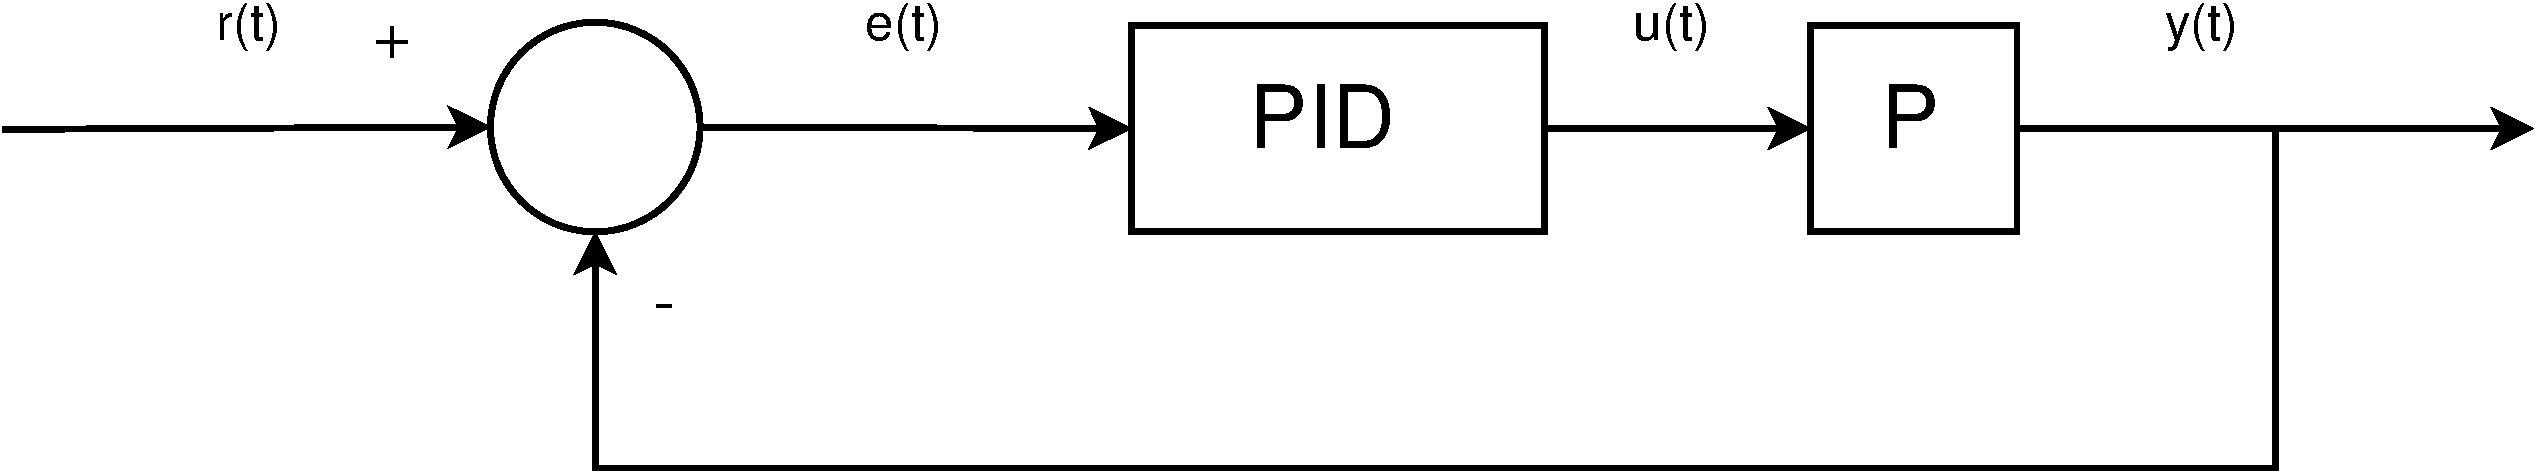
\includegraphics[width=0.8\linewidth]{img/PID}
		\end{figure}
	\end{definition}
	More than 90\% of all closed loop controllers are PID
\end{frame}

\begin{frame}
	\frametitle{What is a PID controller?}
	\begin{itemize}
		\item Proportional action $K_p e(t)$: All advantages of a high loop gain
			\begin{itemize}
				\pro Reduces rise time
				\pro Improves robustness: $K \rightarrow \infty \Rightarrow S^T_P \rightarrow 0$
				\con Reduces but \textbf{does not eliminate steady-state error}: Only when $K \rightarrow \infty , \text{error} \rightarrow 0$
				 (unless plant has pole(s) at $s=0$)
				\con \textbf{Mind stability}: limit on gain
			\end{itemize}
		\pause
		\item Integral action $K_i\int_0^t e(\tau)d\tau$: Reacts on constant errors
			\begin{itemize}
				\pro Augments the type of $P(s)C(s)$ by one, thus \textbf{can eliminate steady state error} in some cases
				\con Makes transient response slower 
			\end{itemize}
		\pause
		\item Derivative action $K_d \frac{de(t)}{dt}$: Reacts on quick variations
		\begin{itemize}
			\pro Damping effect: reduces overshoot, improves transient response
			\con Sensitive for noise, amplifies it if present
		\end{itemize}
	\end{itemize}
\end{frame}

\section{Analog and Digital formulations}

\begin{frame}
	\frametitle{Proportional Control}
	The continuous-time and discrete implementation are identical
	
	Continuous:
	\begin{equation*}
		u_p(t) = K_p e(t) \quad \leftrightarrow \quad \frac{U_p(s)}{E(s)} = K_p 
	\end{equation*}
	Discrete:
	\begin{equation*}
		u_p[k] = K_p e[k] \quad \leftrightarrow \quad \frac{U_p(z)}{E(z)} = K_p 
	\end{equation*}
\end{frame}

\begin{frame}
	\frametitle{Derrivative Control}
	Discretization can be done with \textbf{backward Euler}, applying $\dot{y} \approx \frac{y[k]-y[k-1]}{T}$ or $s = \frac{z - 1}{Tz}$ \\
	Continuous:
	\begin{equation*}
		u_d(t) = K_d \frac{de(t)}{dt} \quad \leftrightarrow \quad \frac{U_d(s)}{E(s)} = K_d s 
	\end{equation*}
	Discrete:
	\begin{equation*}
	u_d[k] = K_d \frac{ e[k] - e[k-1]}{T} \quad \leftrightarrow \quad \frac{U_d(z)}{E(z)} = K_d \frac{z - 1}{Tz}
	\end{equation*}
	with $T$ the sampling time.
	
	Other discretization methods can be used, but forward Euler can introduce instability.
\end{frame}

\begin{frame}
	\frametitle{Integral Control}
	Discretization can be done with \textbf{backward Euler}, applying $\dot{y} \approx \frac{y[k]-y[k-1]}{T}$ or $s = \frac{z - 1}{Tz}$ \\
	The continuous equation is:
	\begin{equation*}
		u_i(t) = K_i \int_0^t e(\tau)d\tau \quad \leftrightarrow \quad \frac{U_i(s)}{E(s)} = \frac{K_i}{p} 
	\end{equation*}
	Differentiating this gives:
	\begin{equation*}
		\dot{u_i} = K_i e(t)
	\end{equation*}
	
	\pause
	Then applying backward Euler:
	\begin{equation*}
	u_i[k] = u[k-1] + K_i T e[k] \quad \leftrightarrow \quad \frac{U_i(z)}{E(z)} =  \frac{K_i T}{1 - z^{-1}}
	\end{equation*}
	with $T$ the sampling time.
	
	Other discretization methods can be used, here is no significant difference.
\end{frame}

\begin{frame}
	\frametitle{Digital formulation combined}
	
	
	\begin{block}{Digital PID controller}
			%Difference equations
			\begin{align*}
			u[k] &= K_p e[k] + \frac{K_d}{T}(e[k] - e[k-1])+u_i[k] \\
			&\text{with } u_i[k] = u_i[k-1] + K_i T e[k]
			\end{align*}
			
			
			In z-domain:
			\begin{equation*}
			\frac{U(z)}{E(z)} = \textcolor{red}{K_p}  + \textcolor{red}{\frac{K_d}{T}}\frac{z-1}{z} + \textcolor{red}{K_i T}\frac{z}{z-1}
			\end{equation*}
			where $\frac{K_d}{T}$ and $K_iT$  are the new derivative and integral gains.
	\end{block}
	
	%\vspace{1em}
	 Also controllers where the integral or derivative function is omitted exist. These are called PI or PD controllers respectively.
\end{frame}

\begin{frame}
	\frametitle{Alternative Digital PID controller }
	We can also discretize using the \textbf{bilinear transformation}:
	\begin{align*}
		\frac{U(z)}{E(z)} &=  
				\left. K_p + \frac{K_i}{s} + K_d s \right|_
							{s=\frac{2}{T}\left( \frac{z-1}{z+1}\right)}  \\
			&= K_p + \frac{K_iT(z + 1)}{2(z-1)} + \frac{2K_d(z-1)}{T(z+1)} \\
			&= \frac{\alpha_2 z^2 + \alpha_1 z + \alpha_0}{(z-1)(z+1)}
	\end{align*}
	
	where $\alpha_2, \alpha_1, \alpha_0$ are design parameters.
	
\end{frame}

\begin{frame}
	\frametitle{Alterantive Derivative Action}
		\begin{columns}
			\begin{column}{0.7\linewidth}
				Imagine a jumping set point or rapidly changing signal. 
				This results in a theoretically infinite, practically very large response of
				the derivative term.  
			\end{column}
			\begin{column}{0.3\linewidth}
				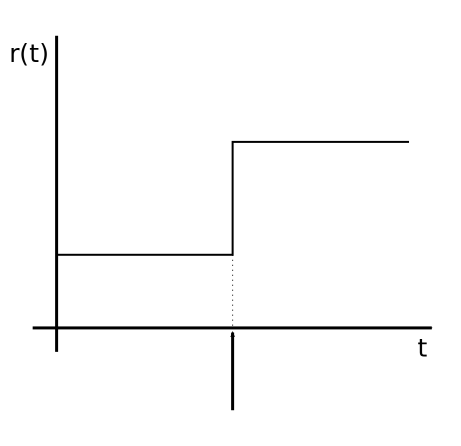
\includegraphics[width=\linewidth]{img/piecewise-setpoint}
			\end{column}
		\end{columns}
		\pause
		$\Rightarrow$ Add a low-pass filter to the derivative term:
		\begin{equation*}
			\frac{U_d(s)}{E(s)} = \frac{K_d s}{1+s\tau}
		\end{equation*}
		With $s=j\omega$, breakpoint at $\omega=1/\tau$. This prevents amplification of high frequencies. 
		
		
		
		
\end{frame}

\begin{frame}
	\frametitle{Alterantive Derivative Action}
	\begin{equation*}
		\frac{U_d(s)}{E(s)} = \frac{K_d s}{1+s\tau}
	\end{equation*}
	
	Further $e(t)$ is replaced by $c\cdot r(t)-y(t)$ with c the set point weighting, which is often set to zero to further reduce immediate influence of a sudden set point jump. 
	
	In time domain:
	
	\begin{equation*}
		u_d(t) = -\tau\frac{du_d}{dt} + K_d(c\cdot r(t)-y(t))
	\end{equation*}
	
	This can also be discretized, but the bilinear method then introduces \emph{ringing}, i.e. large oscillations in transient response.
\end{frame}
\section{Implementation Examples}

\begin{frame}
	\frametitle{Analog Implementation}
	The key building block in the op-amp
	\begin{columns}
		\begin{column}{0.6\linewidth}
			\begin{figure}
				\centering
				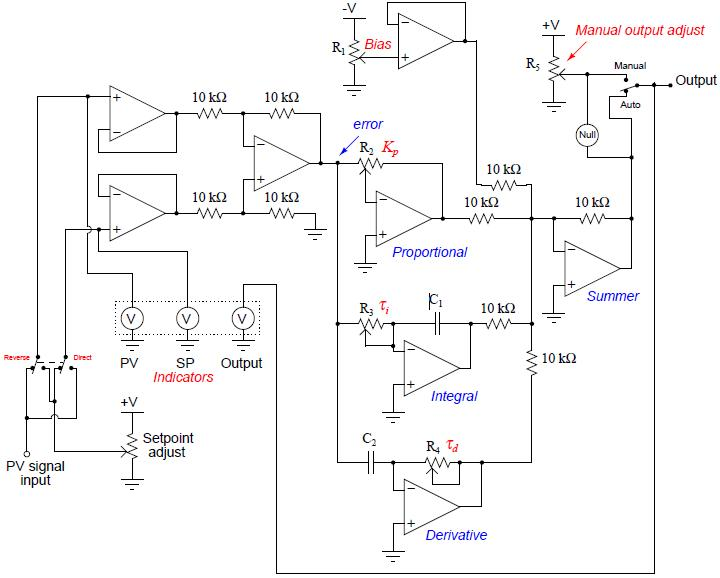
\includegraphics[width=1.1\linewidth]{img/Principles_of_Feedback_Control_Fig_079}
			\end{figure}
		\end{column}
		\begin{column}{0.5\linewidth}
			\begin{itemize}
				\item PV - Process Variable $y(t)$
				\item SP - Set Point $r(t)$
				\item Output - Control action $u(t)$
			\end{itemize}
		\end{column}
	\end{columns}
\end{frame}

\begin{frame}
	\frametitle{Analog Implementation}
	\begin{columns}
		\begin{column}{0.3\linewidth}
			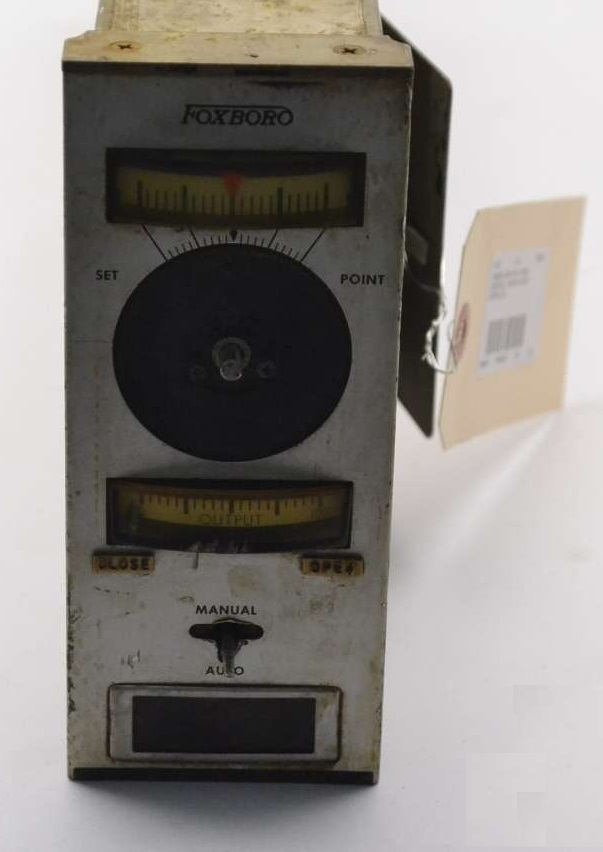
\includegraphics[height=0.6\textheight]{img/FB2a}
		\end{column}
		\begin{column}{0.2\linewidth}
			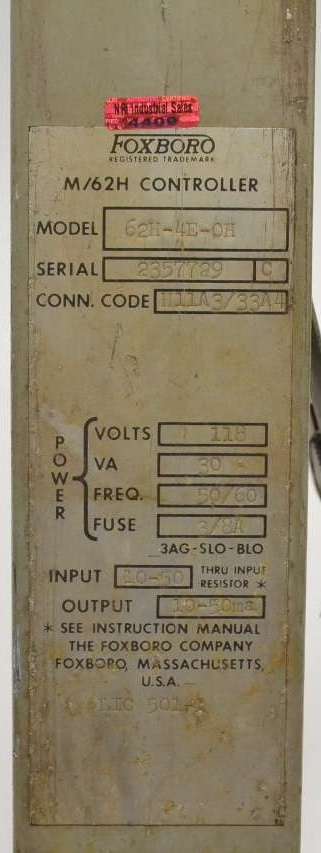
\includegraphics[height=0.6\textheight]{img/fb3a}
		\end{column}
		\begin{column}{0.5\linewidth}
			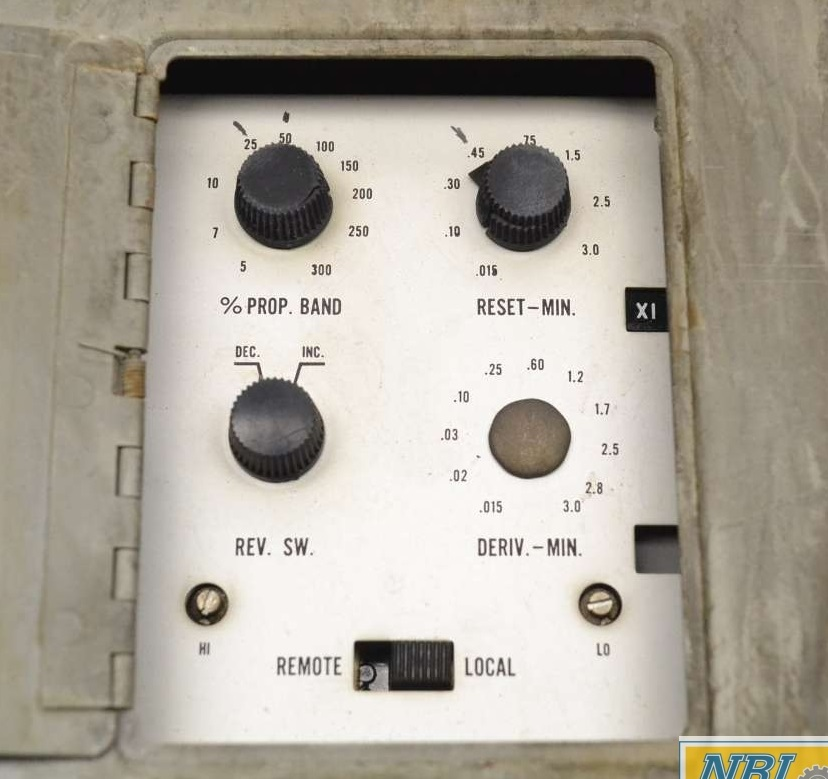
\includegraphics[height=0.6\textheight]{img/fb4}
		\end{column}
	\end{columns}
	\begin{center}
		\textbf{FOXBORO 62H-4E-OH M/62H}
	\end{center}
\end{frame}

\begin{frame}[fragile]
	\frametitle{Digital Implementation}
	The difference equations are typically implemented in a micro controller or FPGA:
		\begin{align*}
		u[k] &= K_p e[k] + \frac{K_d}{T}(e[k] - e[k-1])+u_i[k] \\
		&\text{with } u_i[k] = u_i[k-1] + K_i T e[k]
		\end{align*}
	Steps to be implemented:
	\begin{enumerate}
		\item Wait for clock interrupt
		\item Read analog input
		\item Compute control signal
		\item Set analog output
		\item Update controller variables
		\item Go to 1
	\end{enumerate}
\end{frame}

\begin{frame}
	\frametitle{Digital Implementation Example}
	\begin{columns}
		\begin{column}{0.5\linewidth}
			\centering PLC with a digital PID module:
			
			\vspace{1em}
			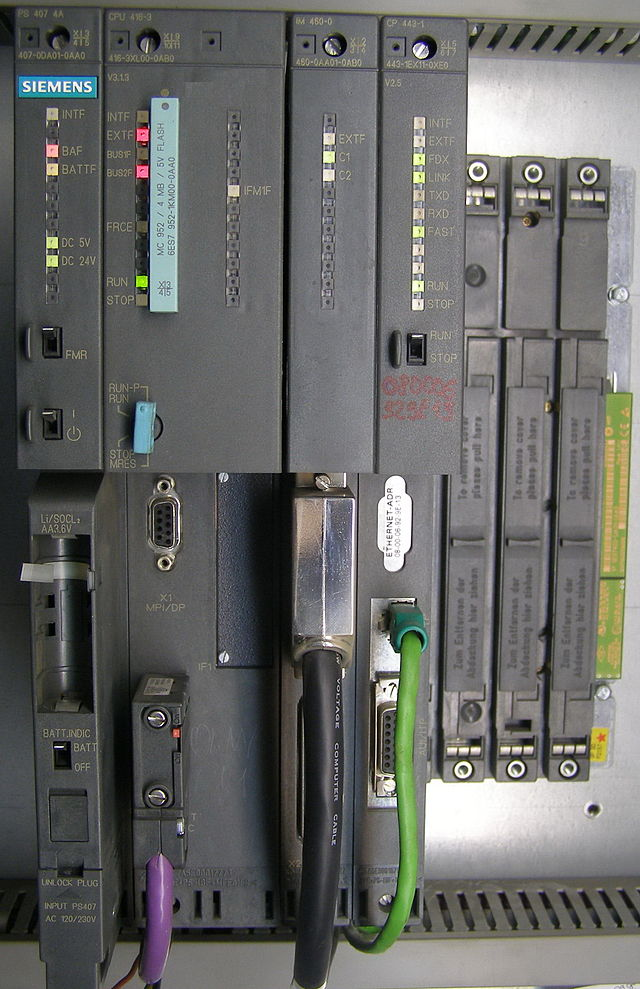
\includegraphics[height=0.7\textheight]{img/640px-Siemens_Simatic_S7-416-3}
		\end{column}
		\begin{column}{0.5\linewidth}
			\centering Digital PID's:
			\vspace{1em}
			\begin{columns}
				\begin{column}{0.4\linewidth}
					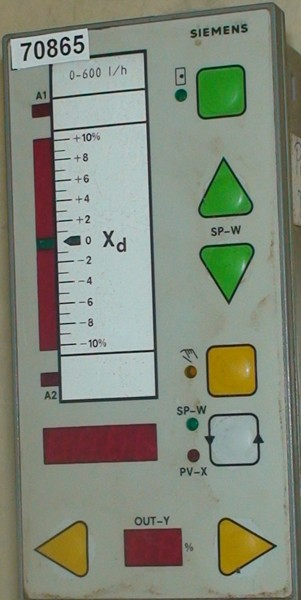
\includegraphics[height=0.7\textheight]{img/278}

				\end{column}
				\begin{column}{0.6\linewidth}
					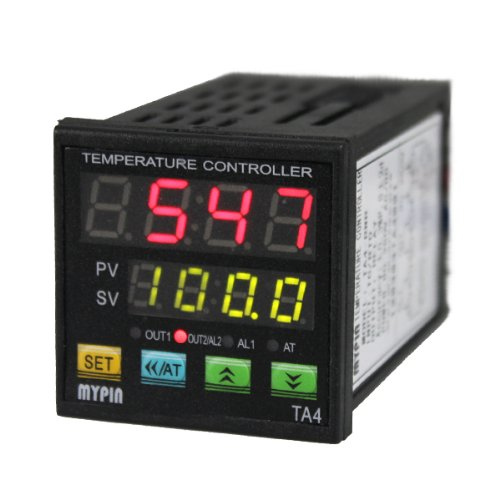
\includegraphics[height=0.4\textheight]{img/41LH64+SGWL}

				\end{column}
			\end{columns}
		\end{column}
	\end{columns}
\end{frame}

\section{PID Tuning}

\begin{frame}
	Effects of adjusting the parameters $K_p, K_i, K_d$:
	\vspace{1em}
	\frametitle{Manual Tuning}
	{
	\small
	\begin{tabular}{c | c | c | c | c }
		PID gains	&	Rise Time 	&	Overshoot	&	Setlling time	&	Steady-State error \\
		\hline
		$K_p \uparrow$ & Decrease	&	Increase	&	Small Change	&	Decrease \\
		$K_i \uparrow$ & Decrease	&	Increase	&	Increase		&	Eliminate \\
		$K_d \uparrow$ & Small change &	Decrease	&	Decrease		&	No change \\
	\end{tabular}
	}
	\vspace{1em}
	
	\textbf{Note:} Changing one parameter can influence the effect of the other two. Use this table only as an indication.
\end{frame}

\begin{frame}
	\frametitle{Manual Tuning}
	In case the controller can be tuned while connected to the plant, following routine can be used:
	\begin{enumerate}
		\item Set $K_i$ and $K_d$ equal to 0
		\item Increase $K_p$ until you observe that the step response is fast enough and the steady-state error in small
		\item Start adding some integral action in order to get rid of the steady state error. Keep in mind that too much $K_i$ can cause instability!
		\item Add some derivative action in order to quickly react to disturbance and/or dampen the response
		
	\end{enumerate}
\end{frame}


\begin{frame}
	\frametitle{Heuristic Methods: Ziegler-Nichols rule}
		This method relies on empirically determining two parameters of the system (should again be practical possible):
		\begin{enumerate}
			\item Set the integral and derivative gains to 0
			\item Increase the proportional gain $K_p$ until the output of the control loop starts oscillating with at constant amplitude. The value of $K_p$ at this point is referred to as ultimate gain $K_u \triangleq K_p$
			\item Measure the period of the oscillations $T_u$ at the output 
		\end{enumerate}
\end{frame}

\begin{frame}
	\frametitle{Heuristic Methods: Ziegler-Nichols rule}
	With $K_u$ and $T_u$ determined like in the previous slide, a starting point for the parameters can be determined:
	\vspace{1em}
	
	\begin{tabular}{c | c | c | c}
		Control Type	&	$K_p$		&	$K_i$			&	$K_d$ 	\\
		\hline
		P				&	$0.5K_u$	&	-				&	-		\\
		PI				&	$0.45K_u$	&	$1.2K_p/T_u$		&	-		\\
		PD				&	$0.8K_u$	&	-				&	$K_pT_u/8$ \\
		PID				&	$0.6K_u$	&	$2K_p/T_u$		&	$K_pT_u/8$ \\
		Pessen Integral Rule & $0.7K_u$ &	$2.5K_p/T_u$	&	$3K_pT_u/20$\\
		Some overshoot	&	$0.33K_u$	&	$2K_p/T_u$		&	$K_pT_u/3$	\\
		No overshoot	&	$0.2K_u$	&	$2K_p/T_u$		&	$K_pT_u/3$	\\
	\end{tabular}
\end{frame}

\begin{frame}
	\frametitle{Numeriacal Optimization Methods}
	
\end{frame}